\documentclass[aspectratio=169]{beamer}

\usetheme{Madrid}
\usecolortheme{default}

\usepackage[utf8]{inputenc}
\usepackage[T1]{fontenc}
\usepackage{amsmath}
\usepackage{graphicx}
\usepackage{booktabs}
\usepackage{xcolor}
\usepackage{tikz}
\usepackage{listings}
\usepackage{algorithm}
\usepackage{algorithmic}

\usetikzlibrary{arrows.meta, positioning, shapes.geometric, calc}

\title[Multimodal Pareto Routing]{Multimodal Pareto-Optimal Path Routing}
\subtitle{A research and engineering view of routing under trade-offs}
\author{Rahul Dev Sharma}
\date{\today}

\definecolor{roadred}{RGB}{210,50,45}
\definecolor{metroblue}{RGB}{45,95,210}
\definecolor{walkgreen}{RGB}{45,150,75}
\definecolor{softgray}{RGB}{238,238,238}
\definecolor{darkgray}{RGB}{70,70,70}
\definecolor{goldnode}{RGB}{245,190,40}
\definecolor{codebg}{RGB}{248,248,248}

\lstset{
    language=Python,
    basicstyle=\ttfamily\scriptsize,
    keywordstyle=\color{metroblue}\bfseries,
    stringstyle=\color{walkgreen!70!black},
    commentstyle=\color{darkgray},
    backgroundcolor=\color{codebg},
    frame=single,
    rulecolor=\color{softgray},
    showstringspaces=false,
    columns=fullflexible,
    keepspaces=true
}

\newcommand{\Rupee}{Rs.\,}
\newcommand{\ImageOrPlaceholder}[2]{%
    \IfFileExists{#1}{%
        \includegraphics[#2]{#1}%
    }{%
        \fbox{\parbox{0.72\textwidth}{\centering
        \vspace{1.1cm}
        \textbf{Image not available}\\[0.15cm]
        \texttt{#1}
        \vspace{1.1cm}}}%
    }%
}

\begin{document}

\begin{frame}
    \titlepage
\end{frame}

% 1. Motivation
\begin{frame}{1. Motivation: Routing Is a Choice Problem}
    \begin{columns}[T]
        \column{0.48\textwidth}
        \begin{block}{A real trip from A to B}
            \begin{itemize}
                \item Cab: fast and direct, but expensive.
                \item Metro: fast over distance, but needs walking.
                \item Walking: free, but slow and tiring.
            \end{itemize}
        \end{block}

        \begin{alertblock}{Why should we care?}
            A route is not just geometry. It reflects time, money, effort, and convenience.
        \end{alertblock}

        \column{0.48\textwidth}
        \centering
        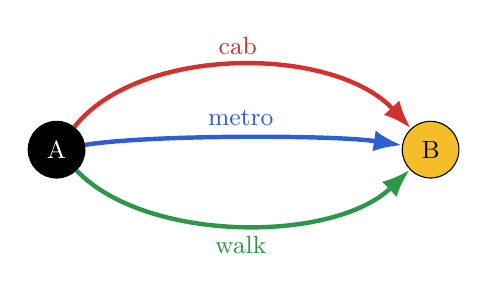
\begin{tikzpicture}[scale=0.95, every node/.style={font=\small}]
            \node[circle, draw, fill=black, text=white, minimum size=0.72cm] (A) at (0,0) {A};
            \node[circle, draw, fill=goldnode, minimum size=0.72cm] (B) at (5,0) {B};
            \draw[roadred, ultra thick, -{Latex}] (A) .. controls (1.1,1.4) and (3.7,1.4) .. node[above] {cab} (B);
            \draw[metroblue, ultra thick, -{Latex}] (A) .. controls (1.2,0.2) and (3.7,0.2) .. node[above] {metro} (B);
            \draw[walkgreen, ultra thick, -{Latex}] (A) .. controls (1.2,-1.25) and (3.7,-1.25) .. node[below] {walk} (B);
        \end{tikzpicture}

        \vspace{0.25cm}
        \begin{block}{Decision dilemma}
            Fast, cheap, low-walk, and low-transfer rarely happen together.
        \end{block}
    \end{columns}
\end{frame}

% 2. Classical Shortest Path
\begin{frame}{2. Classical Shortest Path}
    \begin{columns}[T]
        \column{0.50\textwidth}
        \begin{block}{Intuition: Dijkstra}
            \begin{itemize}
                \item Keep the best known distance to each node.
                \item Expand the node with smallest current distance.
                \item Stop when the destination is finalized.
            \end{itemize}
        \end{block}

        \begin{block}{Small mathematical formulation}
            For scalar edge weight \(w_e\):
            \[
                p^* = \arg\min_{p \in \mathcal{P}_{s,t}}
                \sum_{e \in p} w_e
            \]
        \end{block}

        \column{0.46\textwidth}
        \centering
        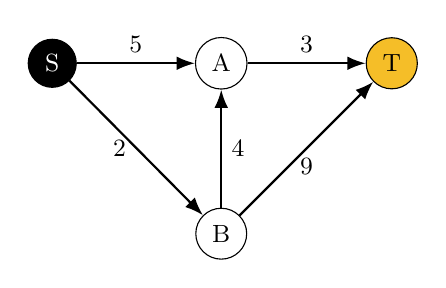
\begin{tikzpicture}[node distance=1.5cm, every node/.style={font=\small}]
            \node[circle, draw, fill=black, text=white] (s) {S};
            \node[circle, draw, right=of s] (a) {A};
            \node[circle, draw, below=of a] (b) {B};
            \node[circle, draw, right=of a, fill=goldnode] (t) {T};
            \draw[-{Latex}, thick] (s) -- node[above] {5} (a);
            \draw[-{Latex}, thick] (s) -- node[left] {2} (b);
            \draw[-{Latex}, thick] (b) -- node[right] {4} (a);
            \draw[-{Latex}, thick] (a) -- node[above] {3} (t);
            \draw[-{Latex}, thick] (b) -- node[below] {9} (t);
        \end{tikzpicture}

        \begin{alertblock}{Limitation}
            Dijkstra assumes one objective represents path quality.
        \end{alertblock}
    \end{columns}
\end{frame}

% 3. Multi-Objective Problem
\begin{frame}{3. Multi-Objective Problem}
    \begin{columns}[T]
        \column{0.48\textwidth}
        \begin{block}{Conflict example}
            \begin{center}
            \begin{tabular}{lcc}
                \toprule
                Path & Time & Cost\\
                \midrule
                A & 20 min & \Rupee 200\\
                B & 30 min & \Rupee 20\\
                \bottomrule
            \end{tabular}
            \end{center}
        \end{block}

        \begin{alertblock}{Which path is better?}
            The answer depends on context. That means scalar ``best'' is not always meaningful.
        \end{alertblock}

        \column{0.48\textwidth}
        \begin{block}{Vector cost}
            Instead of one number, assign each path a vector:
            \[
                C(p) = (C_1(p), C_2(p), \ldots, C_k(p))
            \]
        \end{block}

        \begin{block}{Why care?}
            We can preserve alternatives that are better for different users or situations.
        \end{block}
    \end{columns}
\end{frame}

% 4. Pareto Optimality
\begin{frame}{Why Dijkstra Fails Under Trade-offs}
    \begin{columns}[T]
        \column{0.48\textwidth}
        \begin{block}{Same trip, two valid answers}
            \begin{center}
            \begin{tabular}{lcc}
                \toprule
                Path & Time & Cost\\
                \midrule
                A & 20 min & \Rupee 200\\
                B & 30 min & \Rupee 20\\
                \bottomrule
            \end{tabular}
            \end{center}
        \end{block}

        \begin{alertblock}{Scalar Dijkstra}
            If we force one weighted score, the result depends on the chosen weights.
        \end{alertblock}

        \column{0.48\textwidth}
        \centering
        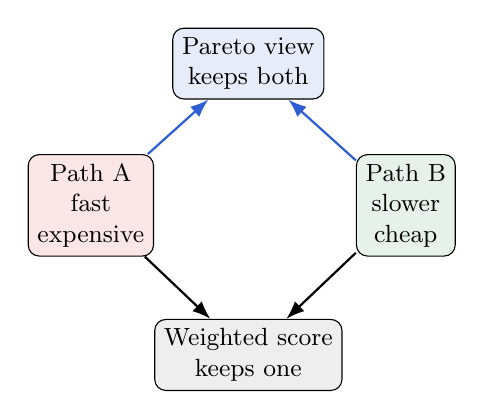
\begin{tikzpicture}[every node/.style={font=\small}]
            \node[draw, rounded corners, fill=roadred!12, align=center] (a) at (0,1.0) {Path A\\fast\\expensive};
            \node[draw, rounded corners, fill=walkgreen!12, align=center] (b) at (4,1.0) {Path B\\slower\\cheap};
            \node[draw, rounded corners, fill=softgray, align=center] (d) at (2,-0.9) {Weighted score\\keeps one};
            \node[draw, rounded corners, fill=metroblue!12, align=center] (p) at (2,2.8) {Pareto view\\keeps both};
            \draw[-{Latex}, thick] (a) -- (d);
            \draw[-{Latex}, thick] (b) -- (d);
            \draw[-{Latex}, thick, metroblue] (a) -- (p);
            \draw[-{Latex}, thick, metroblue] (b) -- (p);
        \end{tikzpicture}

        \begin{block}{Aha}
            The issue is not Dijkstra's mechanics; it is the single-objective assumption.
        \end{block}
    \end{columns}
\end{frame}

\begin{frame}{4. Pareto Optimality: Intuition}
    \begin{block}{Practical rule}
        Keep a route unless another route is no worse in every metric and strictly better in at least one.
    \end{block}

    \begin{columns}[T]
        \column{0.48\textwidth}
        \begin{block}{Two valid paths}
            \begin{itemize}
                \item Path A: faster, more expensive.
                \item Path B: slower, cheaper.
                \item Neither dominates the other.
            \end{itemize}
        \end{block}

        \column{0.48\textwidth}
        \begin{alertblock}{Why care?}
            Pareto optimality prevents us from discarding routes that are useful under different preferences.
        \end{alertblock}
    \end{columns}
\end{frame}

\begin{frame}{4. Pareto Optimality: Diagram}
    \centering
    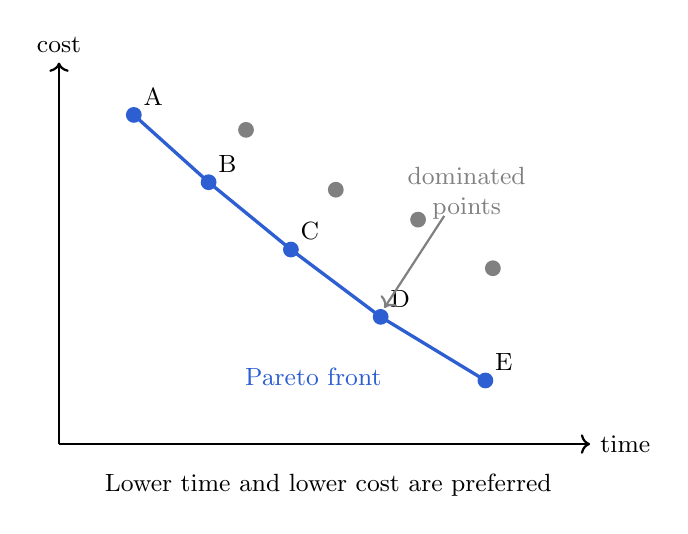
\begin{tikzpicture}[scale=0.95, every node/.style={font=\small}]
        \draw[->, thick] (0,0) -- (7.1,0) node[right] {time};
        \draw[->, thick] (0,0) -- (0,5.1) node[above] {cost};

        \foreach \x/\y/\name in {1.0/4.4/A,2.0/3.5/B,3.1/2.6/C,4.3/1.7/D,5.7/0.85/E} {
            \fill[metroblue] (\x,\y) circle (3pt);
            \node[above right] at (\x,\y) {\name};
        }
        \draw[metroblue, very thick] (1.0,4.4) -- (2.0,3.5) -- (3.1,2.6) -- (4.3,1.7) -- (5.7,0.85);

        \foreach \x/\y in {2.5/4.2,3.7/3.4,4.8/3.0,5.8/2.35} {
            \fill[gray] (\x,\y) circle (3pt);
        }
        \node[metroblue] at (3.4,0.9) {Pareto front};
        \node[gray, align=center] at (5.45,3.35) {dominated\\points};
        \draw[->, gray, thick] (5.15,3.05) -- (4.35,1.82);
        \node at (3.6,-0.55) {Lower time and lower cost are preferred};
    \end{tikzpicture}
\end{frame}

\begin{frame}{4. Pareto Optimality: Formal Rule}
    \begin{block}{Dominance}
        Path \(p\) dominates path \(q\) when:
    \end{block}

    \[
        \forall i,\; C_i(p) \le C_i(q),
        \qquad
        \exists j:\ C_j(p) < C_j(q)
    \]

    \begin{block}{Non-dominated set}
        The Pareto set contains paths that are not dominated by any other feasible path.
    \end{block}

    \begin{alertblock}{Engineering meaning}
        This rule gives a deterministic filter for keeping useful alternatives.
    \end{alertblock}
\end{frame}

% 5. Problem Formulation
\begin{frame}{5. Problem Formulation}
    \begin{block}{Path profile}
        In this project, each path is represented as:
        \[
            C(p) = (t,\ w,\ tr,\ c)
        \]
    \end{block}

    \begin{columns}[T]
        \column{0.48\textwidth}
        \begin{itemize}
            \item \(t\): total travel time.
            \item \(w\): walking distance.
            \item \(tr\): number of transfers.
            \item \(c\): monetary cost.
        \end{itemize}

        \column{0.48\textwidth}
        \begin{block}{Example route}
            Walk to metro, ride metro, then use road:
            \[
                (25.3\text{ min},\ 1.2\text{ km},\ 2,\ \Rupee 42.5)
            \]
        \end{block}
    \end{columns}

    \begin{alertblock}{Goal}
        Compute bounded Pareto-optimal paths and return diverse Top-\(K\) representatives.
    \end{alertblock}
\end{frame}

% 6. System Pipeline
\begin{frame}[shrink=8]{6. System Pipeline}
    \centering
    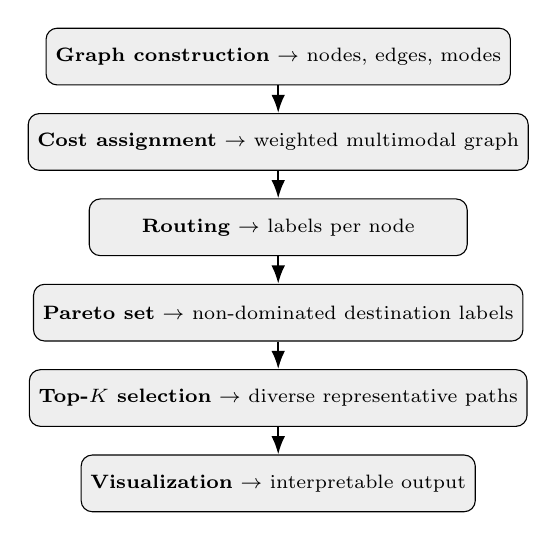
\begin{tikzpicture}[
        node distance=0.35cm,
        stage/.style={draw, rounded corners, align=left, fill=softgray, minimum width=4.8cm, minimum height=0.72cm, font=\scriptsize},
        arrow/.style={-{Latex}, thick}
    ]
        \node[stage] (g) {\textbf{Graph construction} \(\rightarrow\) nodes, edges, modes};
        \node[stage, below=of g] (cost) {\textbf{Cost assignment} \(\rightarrow\) weighted multimodal graph};
        \node[stage, below=of cost] (route) {\textbf{Routing} \(\rightarrow\) labels per node};
        \node[stage, below=of route] (pareto) {\textbf{Pareto set} \(\rightarrow\) non-dominated destination labels};
        \node[stage, below=of pareto] (topk) {\textbf{Top-\(K\) selection} \(\rightarrow\) diverse representative paths};
        \node[stage, below=of topk] (vis) {\textbf{Visualization} \(\rightarrow\) interpretable output};

        \draw[arrow] (g) -- (cost);
        \draw[arrow] (cost) -- (route);
        \draw[arrow] (route) -- (pareto);
        \draw[arrow] (pareto) -- (topk);
        \draw[arrow] (topk) -- (vis);
    \end{tikzpicture}

    \vspace{0.1cm}
    \begin{block}{End-to-end view}
        The data structure evolves from a graph, to labels, to non-dominated paths, to a small visual decision set.
    \end{block}
\end{frame}

% 7. Synthetic Network
\begin{frame}{7. Synthetic Network}
    \begin{columns}[T]
        \column{0.42\textwidth}
        \begin{block}{Network structure}
            \begin{itemize}
                \item Grid road network.
                \item Straight metro lines.
                \item Walking links between nearby nodes.
                \item Parallel edges allowed for different modes.
            \end{itemize}
        \end{block}

        \begin{alertblock}{Why synthetic?}
            It gives controlled trade-offs and repeatable experiments.
        \end{alertblock}

        \column{0.54\textwidth}
        \centering
        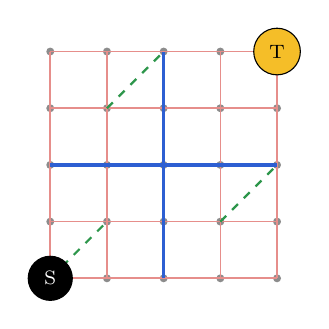
\begin{tikzpicture}[scale=0.72, every node/.style={font=\scriptsize}]
            \foreach \x in {0,...,4} {
                \foreach \y in {0,...,4} {
                    \fill[black!45] (\x,\y) circle (2pt);
                }
            }
            \foreach \x in {0,...,4} {
                \draw[roadred!55, line width=0.6pt] (\x,0) -- (\x,4);
            }
            \foreach \y in {0,...,4} {
                \draw[roadred!55, line width=0.6pt] (0,\y) -- (4,\y);
            }
            \draw[metroblue, very thick] (0,2) -- (4,2);
            \draw[metroblue, very thick] (2,0) -- (2,4);
            \draw[walkgreen, dashed, thick] (0,0) -- (1,1);
            \draw[walkgreen, dashed, thick] (3,1) -- (4,2);
            \draw[walkgreen, dashed, thick] (1,3) -- (2,4);
            \node[draw, fill=black, text=white, circle] at (0,0) {S};
            \node[draw, fill=goldnode, circle] at (4,4) {T};
        \end{tikzpicture}
    \end{columns}
\end{frame}

% 8. Cost Modeling
\begin{frame}{8. Cost Modeling}
    \begin{columns}[T]
        \column{0.48\textwidth}
        \begin{block}{Road}
            Road cost accounts for distance, fuel, time value, and congestion:
            \[
                c_{\text{road}} =
                \frac{d}{m}\,f + \gamma t + \delta\rho
            \]
            \scriptsize
            \(d\): distance, \(m\): mileage, \(f\): fuel price, \(\rho\): congestion penalty.
        \end{block}

        \column{0.48\textwidth}
        \begin{block}{Metro and walking}
            Metro fare:
            \[
                c_{\text{metro}} = \alpha + \beta d
            \]
            Walking:
            \[
                c_{\text{walk}} = 0
            \]
        \end{block}
    \end{columns}

    \begin{alertblock}{Why care?}
        Mode-dependent costs create realistic conflicts between fast, cheap, and low-effort paths.
    \end{alertblock}
\end{frame}

% 9. Core Algorithm
\begin{frame}{9. Multi-Objective Label Setting: Intuition}
    \begin{columns}[T]
        \column{0.47\textwidth}
        \begin{block}{Classical shortest path}
            One best label per node.
        \end{block}

        \begin{block}{Multi-objective version}
            Keep multiple labels when they represent different trade-offs.
        \end{block}

        \column{0.49\textwidth}
        \centering
        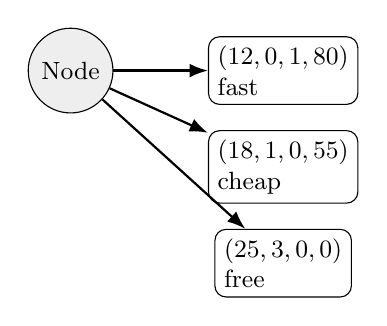
\begin{tikzpicture}[every node/.style={font=\small}]
            \node[circle, draw, fill=softgray, minimum size=1.0cm] (n) at (0,0) {Node};
            \node[draw, rounded corners, right=1.2cm of n, align=left] (l1) {\((12,0,1,80)\)\\fast};
            \node[draw, rounded corners, below=0.32cm of l1, align=left] (l2) {\((18,1,0,55)\)\\cheap};
            \node[draw, rounded corners, below=0.32cm of l2, align=left] (l3) {\((25,3,0,0)\)\\free};
            \draw[-{Latex}, thick] (n) -- (l1);
            \draw[-{Latex}, thick] (n) -- (l2);
            \draw[-{Latex}, thick] (n) -- (l3);
        \end{tikzpicture}
    \end{columns}

    \begin{alertblock}{Key intuition}
        A partial path that is not fastest may still become the cheapest or simplest complete route.
    \end{alertblock}
\end{frame}

\begin{frame}{What Happens Internally}
    \begin{columns}[T]
        \column{0.45\textwidth}
        \begin{block}{Graph becomes a state space}
            The algorithm does not only ask ``which node am I at?'' It asks:
            \[
                \text{node} + \text{current trade-off vector}
            \]
        \end{block}

        \begin{block}{Each node holds a frontier}
            A node may store several labels because each label represents a different way to arrive there.
        \end{block}

        \column{0.51\textwidth}
        \centering
        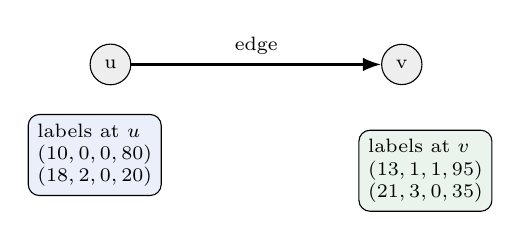
\begin{tikzpicture}[every node/.style={font=\scriptsize}]
            \node[circle, draw, fill=softgray] (u) at (0,0) {u};
            \node[circle, draw, fill=softgray] (v) at (3.7,0) {v};
            \draw[-{Latex}, thick] (u) -- node[above] {edge} (v);
            \node[draw, rounded corners, align=left, fill=metroblue!10] at (-0.2,-1.15) {
                labels at \(u\)\\
                \((10,0,0,80)\)\\
                \((18,2,0,20)\)
            };
            \node[draw, rounded corners, align=left, fill=walkgreen!10] at (4.0,-1.35) {
                labels at \(v\)\\
                \((13,1,1,95)\)\\
                \((21,3,0,35)\)
            };
        \end{tikzpicture}

        \begin{alertblock}{Aha}
            The algorithm explores the frontier of trade-offs, not just the frontier of nodes.
        \end{alertblock}
    \end{columns}
\end{frame}

\begin{frame}{9. Multi-Objective Label Setting: Mathematical Idea}
    \begin{block}{Label}
        A label at node \(v\) stores a cost vector and predecessor:
        \[
            L = (v,\ C_L,\ \text{prev},\ \text{mode},\ \text{route\_id})
        \]
    \end{block}

    \begin{block}{Propagation over edge \(e=(u,v)\)}
        If \(L\) is a label at \(u\), generate:
        \[
            C_{L'} = C_L + C_e + (0,0,\Delta tr,0)
        \]
        where \(\Delta tr=1\) if the mode or transit route changes.
    \end{block}

    \begin{alertblock}{Engineering rule}
        Keep \(L'\) only if it is feasible and not dominated at node \(v\).
    \end{alertblock}
\end{frame}

\begin{frame}[shrink=12]{9. Multi-Objective Label Setting: Pseudocode}
    \scriptsize
    \begin{algorithm}[H]
    \caption{Multi-objective Label Setting}
    \begin{algorithmic}[1]
        \STATE Initialize labels at source \(s\)
        \STATE Push source label into priority queue
        \WHILE{queue not empty}
            \STATE Extract label \(L\)
            \FOR{each outgoing edge \(e=(L.node,v)\)}
                \STATE Generate new label \(L'\)
                \STATE Apply feasibility bounds
                \STATE Apply dominance check at node \(v\)
                \IF{\(L'\) is feasible and non-dominated}
                    \STATE Insert \(L'\); remove labels dominated by \(L'\)
                \ENDIF
            \ENDFOR
        \ENDWHILE
        \STATE Return active labels at destination
    \end{algorithmic}
    \end{algorithm}
\end{frame}

\begin{frame}{How the Algorithm Builds a Path}
    \begin{columns}[T]
        \column{0.48\textwidth}
        \begin{block}{Step-by-step expansion}
            \begin{itemize}
                \item Start at source: \((0,0,0,0)\)
                \item Expand via road: \((5,0,0,20)\)
                \item Expand via metro: \((3,1,1,15)\)
                \item Compare: both are non-dominated, so keep both.
                \item Continue expansion from both labels.
            \end{itemize}
        \end{block}

        \column{0.48\textwidth}
        \centering
        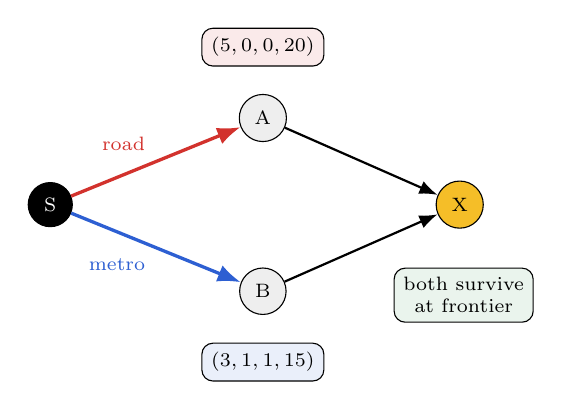
\begin{tikzpicture}[every node/.style={font=\scriptsize}]
            \node[circle, draw, fill=black, text=white] (s) at (0,0) {S};
            \node[circle, draw, fill=softgray] (a) at (2.7,1.1) {A};
            \node[circle, draw, fill=softgray] (b) at (2.7,-1.1) {B};
            \node[circle, draw, fill=goldnode] (x) at (5.2,0) {X};
            \draw[-{Latex}, roadred, very thick] (s) -- node[above left] {road} (a);
            \draw[-{Latex}, metroblue, very thick] (s) -- node[below left] {metro} (b);
            \draw[-{Latex}, thick] (a) -- (x);
            \draw[-{Latex}, thick] (b) -- (x);
            \node[draw, rounded corners, fill=roadred!10, align=left] at (2.7,2.0) {\((5,0,0,20)\)};
            \node[draw, rounded corners, fill=metroblue!10, align=left] at (2.7,-2.0) {\((3,1,1,15)\)};
            \node[draw, rounded corners, fill=walkgreen!10, align=center] at (5.25,-1.15) {both survive\\at frontier};
        \end{tikzpicture}
    \end{columns}
\end{frame}

% 10. Dominance
\begin{frame}{10. Dominance: Visual and Math}
    \begin{columns}[T]
        \column{0.42\textwidth}
        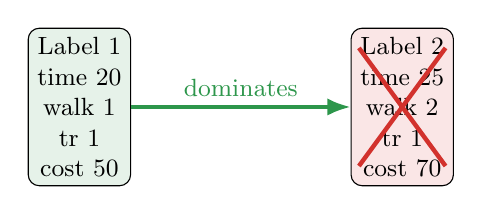
\begin{tikzpicture}[every node/.style={font=\small}]
            \node[draw, rounded corners, fill=walkgreen!12, align=center] (good) at (0,1.1) {
                Label 1\\
                time 20\\walk 1\\tr 1\\cost 50
            };
            \node[draw, rounded corners, fill=roadred!12, align=center] (bad) at (4.1,1.1) {
                Label 2\\
                time 25\\walk 2\\tr 1\\cost 70
            };
            \draw[-{Latex}, very thick, walkgreen] (good) -- node[above] {dominates} (bad);
            \draw[roadred, ultra thick] (3.55,0.35) -- (4.65,1.85);
            \draw[roadred, ultra thick] (4.65,0.35) -- (3.55,1.85);
        \end{tikzpicture}

        \column{0.54\textwidth}
        \begin{block}{Why Label 1 dominates}
            \begin{itemize}
                \item \(\checkmark\) better in time: \(20 < 25\)
                \item \(\checkmark\) better in walking: \(1 < 2\)
                \item \(\checkmark\) equal in transfers: \(1 = 1\)
                \item \(\checkmark\) better in cost: \(50 < 70\)
            \end{itemize}
        \end{block}

        \begin{block}{Formal dominance}
            \[
                \forall i,\ C_i(a)\le C_i(b),
                \quad
                \exists j:\ C_j(a)<C_j(b)
            \]
        \end{block}

        \begin{alertblock}{Why care?}
            Dominance is the main correctness rule for pruning bad labels without scalarization.
        \end{alertblock}
    \end{columns}
\end{frame}

% 11. Pruning Strategy
\begin{frame}{Failure Without Pruning}
    \begin{columns}[T]
        \column{0.48\textwidth}
        \begin{block}{Label explosion}
            Without pruning, small trade-offs can create many labels:
            \[
            \begin{array}{c}
            (10,1,1,100)\\
            (11,1,1,99)\\
            (12,1,1,98)\\
            (13,1,1,97)\\
            \vdots
            \end{array}
            \]
        \end{block}

        \column{0.48\textwidth}
        \begin{alertblock}{Why this is dangerous}
            \begin{itemize}
                \item More labels per node.
                \item More queue operations.
                \item More dominance comparisons.
                \item Slower search and harder interpretation.
            \end{itemize}
        \end{alertblock}

        \begin{block}{Aha}
            Pareto routing needs both correctness and control.
        \end{block}
    \end{columns}
\end{frame}

\begin{frame}{11. Pruning Strategy}
    \begin{columns}[T]
        \column{0.47\textwidth}
        \begin{block}{Why needed}
            Multi-objective routing can create many labels because different partial paths are incomparable.
        \end{block}

        \begin{block}{Feasibility bounds}
            \[
                t \le \alpha_t t^*,
                \quad
                w \le \alpha_w w^*,
                \quad
                c \le \alpha_c c^*
            \]
            Also enforce \(tr \le \alpha_{tr}\).
        \end{block}

        \column{0.49\textwidth}
        \begin{block}{Interpretation}
            \begin{itemize}
                \item \(t^*, w^*, c^*\): single-objective best values.
                \item \(\alpha\)'s control tolerance.
                \item Bounds remove unrealistic detours.
            \end{itemize}
        \end{block}

        \begin{alertblock}{Balance}
            Tight bounds are fast but may hide alternatives; loose bounds reveal more but cost more.
        \end{alertblock}
    \end{columns}
\end{frame}

\begin{frame}{Trade-off Between Accuracy and Speed}
    \begin{columns}[T]
        \column{0.45\textwidth}
        \begin{block}{Tight bounds}
            \begin{itemize}
                \item Faster runtime.
                \item Fewer labels.
                \item May miss some alternatives.
            \end{itemize}
        \end{block}

        \begin{block}{Loose bounds}
            \begin{itemize}
                \item Richer Pareto set.
                \item More labels.
                \item Slower runtime.
            \end{itemize}
        \end{block}

        \column{0.51\textwidth}
        \centering
        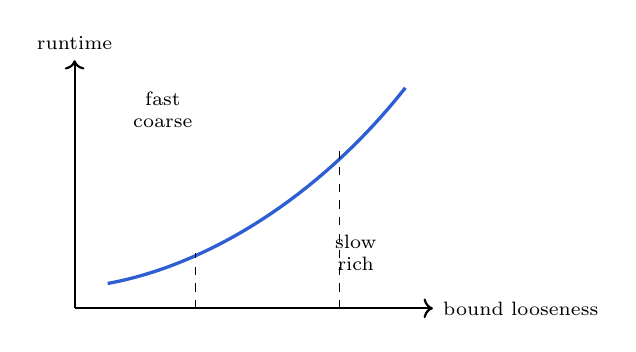
\begin{tikzpicture}[scale=0.70, every node/.style={font=\scriptsize}]
            \draw[->, thick] (0,0) -- (6.5,0) node[right] {bound looseness};
            \draw[->, thick] (0,0) -- (0,4.5) node[above] {runtime};
            \draw[metroblue, very thick] (0.6,0.45) .. controls (2.5,0.8) and (4.5,2.1) .. (6.0,4.0);
            \node[align=center] at (1.6,3.6) {fast\\coarse};
            \node[align=center] at (5.1,1.0) {slow\\rich};
            \draw[dashed] (2.2,0) -- (2.2,1.0);
            \draw[dashed] (4.8,0) -- (4.8,2.9);
        \end{tikzpicture}
    \end{columns}
\end{frame}

\begin{frame}{Complexity Analysis}
    \begin{columns}[T]
        \column{0.48\textwidth}
        \begin{block}{Classical Dijkstra}
            One label per node:
            \[
                O((V+E)\log V)
            \]
        \end{block}

        \begin{block}{Multi-objective label setting}
            Let \(L\) be the average number of labels per node:
            \[
                O\!\left(L\cdot(V+E)\log(LV)\right)
            \]
        \end{block}

        \column{0.48\textwidth}
        \begin{alertblock}{Important insight}
            Worst case can be exponential in the number of objectives because many labels may be mutually non-dominated.
        \end{alertblock}

        \begin{block}{Practical case}
            Dominance checks, feasibility bounds, and Top-\(K\) post-selection keep \(L\) manageable.
        \end{block}
    \end{columns}
\end{frame}

% 12. Diversity-Based Selection
\begin{frame}{12. Diversity-Based Top-\(K\) Selection}
    \begin{columns}[T]
        \column{0.47\textwidth}
        \begin{block}{Why Top-\(K\)?}
            A Pareto set can contain many valid paths. Users need a compact set of distinct choices.
        \end{block}

        \begin{block}{Selection idea}
            Start with anchors: min time, min walk, min transfers, min cost.
            Then add paths that are far from already selected paths.
        \end{block}

        \column{0.49\textwidth}
        \begin{block}{Max-min rule}
            \[
                p^* = \arg\max_{p \in P\setminus S}
                \min_{q \in S} d(p,q)
            \]
            \[
                d(p,q)=|\Delta t|+|\Delta w|+|\Delta tr|+|\Delta c|
            \]
        \end{block}

        \begin{alertblock}{Why care?}
            We present diverse trade-offs rather than several nearly identical paths.
        \end{alertblock}
    \end{columns}
\end{frame}

% 13. Implementation
\begin{frame}[shrink=8]{Algorithm \(\rightarrow\) Code Mapping}
    \begin{block}{Bridge from theory to implementation}
        Each algorithmic concept is represented by a small, testable code unit.
    \end{block}

    \begin{center}
    \begin{tabular}{ll}
        \toprule
        \textbf{Concept} & \textbf{Code representation}\\
        \midrule
        Label & \texttt{class Label}\\
        Cost vector & \texttt{(time, walk, transfers, cost)}\\
        Dominance & \texttt{dominates(a, b)}\\
        Expansion & edge attribute update\\
        Queue & \texttt{heapq} priority queue\\
        Path reconstruction & predecessor pointers\\
        Top-\(K\) diversity & greedy max-min selector\\
        \bottomrule
    \end{tabular}
    \end{center}

    \begin{alertblock}{Why care?}
        This mapping keeps the implementation modular: graph building, routing, Pareto utilities, diversity, and visualization remain separate.
    \end{alertblock}
\end{frame}

\begin{frame}[fragile]{13. Implementation: Label Structure}
    \begin{block}{Code idea}
        Each label stores the node, objective vector, and predecessor pointer for reconstruction.
    \end{block}

\begin{lstlisting}[language=Python]
class Label:
    def __init__(self, node, costs, prev=None,
                 previous_mode=None, route_id=None):
        self.node = node
        self.costs = costs      # (time, walk, transfers, cost)
        self.prev = prev
        self.previous_mode = previous_mode
        self.route_id = route_id
        self.active = True
\end{lstlisting}

    \begin{alertblock}{Why care?}
        The predecessor pointer turns final labels back into complete paths.
    \end{alertblock}
\end{frame}

\begin{frame}[fragile]{13. Implementation: Dominance Check}
    \begin{block}{Short and exact}
        Dominance is implemented directly from the mathematical definition.
    \end{block}

\begin{lstlisting}[language=Python]
def dominates(a, b):
    return (
        all(x <= y for x, y in zip(a, b)) and
        any(x < y for x, y in zip(a, b))
    )
\end{lstlisting}

    \begin{block}{Usage}
        Before adding a new label, compare it with active labels at the same node.
    \end{block}
\end{frame}

\begin{frame}[fragile]{13. Implementation: Edge Expansion}
    \begin{block}{Core engineering step}
        Extend a label through an outgoing edge and update transfer count.
    \end{block}

\begin{lstlisting}[language=Python]
new_costs = (
    costs[0] + edge["time"],
    costs[1] + edge["walk"],
    costs[2] + transfer_increment,
    costs[3] + edge["cost"],
)
\end{lstlisting}

    \begin{alertblock}{Important}
        The algorithm never collapses objectives into a weighted sum.
    \end{alertblock}
\end{frame}

% 14. Visualization
\begin{frame}{14. Visualization}
    \begin{columns}[T]
        \column{0.40\textwidth}
        \begin{block}{Color mapping}
            \begin{itemize}
                \item \textcolor{roadred}{Red}: road
                \item \textcolor{metroblue}{Blue}: metro
                \item \textcolor{walkgreen}{Green}: walk
            \end{itemize}
        \end{block}

        \begin{block}{Drawing rule}
            Draw each consecutive path segment using the edge's mode.
        \end{block}

        \column{0.56\textwidth}
        \begin{figure}
            \centering
            \ImageOrPlaceholder{images/all_paths.png}{width=0.95\textwidth}
            \caption{Mode-colored Top-\(K\) paths.}
        \end{figure}
    \end{columns}
\end{frame}

% 15. Results
\begin{frame}{15. Results: All Selected Paths}
    \begin{figure}
        \centering
        \ImageOrPlaceholder{images/all_paths.png}{height=0.70\textheight}
        \caption{All selected Pareto paths overlaid on the network.}
    \end{figure}
\end{frame}

\begin{frame}[shrink=8]{15. Results: Path 1}
    \begin{columns}[T]
        \column{0.66\textwidth}
        \begin{figure}
            \centering
            \ImageOrPlaceholder{images/path_1.png}{width=0.84\textwidth}
            \caption{Path 1}
        \end{figure}
        \column{0.30\textwidth}
        \begin{alertblock}{Interpretation}
            Fastest representative path, but expensive and transfer-heavy.
        \end{alertblock}
        \begin{block}{Metrics}
            Time: 12.27 min\\
            Walk: 0.00 km\\
            Transfers: 4\\
            Cost: \Rupee 101.39
        \end{block}
        \begin{block}{Why Pareto?}
            Faster than cheaper paths; not dominated despite higher cost.
        \end{block}
    \end{columns}
\end{frame}

\begin{frame}[shrink=8]{15. Results: Path 2}
    \begin{columns}[T]
        \column{0.66\textwidth}
        \begin{figure}
            \centering
            \ImageOrPlaceholder{images/path_2.png}{width=0.84\textwidth}
            \caption{Path 2}
        \end{figure}
        \column{0.30\textwidth}
        \begin{alertblock}{Interpretation}
            Road-only path: simple and no transfers, but still costly.
        \end{alertblock}
        \begin{block}{Metrics}
            Time: 18.72 min\\
            Walk: 0.00 km\\
            Transfers: 0\\
            Cost: \Rupee 96.68
        \end{block}
        \begin{block}{Why Pareto?}
            Fewer transfers than faster paths; faster than cheaper paths.
        \end{block}
    \end{columns}
\end{frame}

\begin{frame}[shrink=8]{15. Results: Path 3}
    \begin{columns}[T]
        \column{0.66\textwidth}
        \begin{figure}
            \centering
            \ImageOrPlaceholder{images/path_3.png}{width=0.84\textwidth}
            \caption{Path 3}
        \end{figure}
        \column{0.30\textwidth}
        \begin{alertblock}{Interpretation}
            Walking-only path: zero cost and zero transfers, but slow.
        \end{alertblock}
        \begin{block}{Metrics}
            Time: 96.00 min\\
            Walk: 8.00 km\\
            Transfers: 0\\
            Cost: \Rupee 0.00
        \end{block}
        \begin{block}{Why Pareto?}
            No other path is cheaper; cost anchors the frontier.
        \end{block}
    \end{columns}
\end{frame}

\begin{frame}[shrink=8]{15. Results: Path 4}
    \begin{columns}[T]
        \column{0.66\textwidth}
        \begin{figure}
            \centering
            \ImageOrPlaceholder{images/path_4.png}{width=0.84\textwidth}
            \caption{Path 4}
        \end{figure}
        \column{0.30\textwidth}
        \begin{alertblock}{Interpretation}
            Balanced cost-time option with moderate walking.
        \end{alertblock}
        \begin{block}{Metrics}
            Time: 55.87 min\\
            Walk: 4.00 km\\
            Transfers: 4\\
            Cost: \Rupee 46.75
        \end{block}
        \begin{block}{Why Pareto?}
            Cheaper than faster paths; faster than lower-cost walking-heavy paths.
        \end{block}
    \end{columns}
\end{frame}

\begin{frame}[shrink=8]{15. Results: Path 5}
    \begin{columns}[T]
        \column{0.66\textwidth}
        \begin{figure}
            \centering
            \ImageOrPlaceholder{images/path_5.png}{width=0.84\textwidth}
            \caption{Path 5}
        \end{figure}
        \column{0.30\textwidth}
        \begin{alertblock}{Interpretation}
            Faster than walking-heavy routes, cheaper than road-heavy routes.
        \end{alertblock}
        \begin{block}{Metrics}
            Time: 35.50 min\\
            Walk: 2.00 km\\
            Transfers: 4\\
            Cost: \Rupee 71.84
        \end{block}
        \begin{block}{Why Pareto?}
            Occupies the middle: lower cost than fast road-heavy routes with less walking than cheap routes.
        \end{block}
    \end{columns}
\end{frame}

\begin{frame}[shrink=8]{15. Results: Path 6}
    \begin{columns}[T]
        \column{0.66\textwidth}
        \begin{figure}
            \centering
            \ImageOrPlaceholder{images/path_6.png}{width=0.84\textwidth}
            \caption{Path 6}
        \end{figure}
        \column{0.30\textwidth}
        \begin{alertblock}{Interpretation}
            Low-cost alternative with more walking and longer travel time.
        \end{alertblock}
        \begin{block}{Metrics}
            Time: 76.33 min\\
            Walk: 6.00 km\\
            Transfers: 4\\
            Cost: \Rupee 22.18
        \end{block}
        \begin{block}{Why Pareto?}
            Much cheaper than faster routes; faster than the zero-cost walking-only route.
        \end{block}
    \end{columns}
\end{frame}

\begin{frame}{15. Results: Time-Cost Pareto Front}
    \begin{figure}
        \centering
        \ImageOrPlaceholder{images/pareto_front.png}{height=0.70\textheight}
        \caption{Computed Pareto frontier in time-cost space.}
    \end{figure}
\end{frame}

\begin{frame}{Insights from Results}
    \begin{columns}[T]
        \column{0.32\textwidth}
        \begin{block}{Fast paths}
            \begin{itemize}
                \item Low time.
                \item Higher cost.
                \item Often more mode changes.
            \end{itemize}
        \end{block}

        \column{0.32\textwidth}
        \begin{block}{Cheap paths}
            \begin{itemize}
                \item Low or zero cost.
                \item More walking.
                \item Longer travel time.
            \end{itemize}
        \end{block}

        \column{0.32\textwidth}
        \begin{block}{Balanced paths}
            \begin{itemize}
                \item Moderate cost.
                \item Moderate walking.
                \item Useful compromise.
            \end{itemize}
        \end{block}
    \end{columns}

    \begin{alertblock}{Aha}
        The visualization is not just decorative: it explains why the Pareto set has structure.
    \end{alertblock}
\end{frame}

% 16. Key Insights
\begin{frame}{16. Key Insights}
    \begin{columns}[T]
        \column{0.48\textwidth}
        \begin{block}{Routing insight}
            There is often no single best route under multiple objectives.
        \end{block}

        \begin{block}{Algorithmic insight}
            Multi-objective labels preserve trade-offs that scalar shortest path algorithms discard.
        \end{block}

        \column{0.48\textwidth}
        \begin{alertblock}{System insight}
            Pareto filtering plus Top-\(K\) diversity turns a large solution set into actionable choices.
        \end{alertblock}

        \begin{block}{User insight}
            Travelers can compare fast, cheap, low-walk, and low-transfer options explicitly.
        \end{block}
    \end{columns}
\end{frame}

% 17. Conclusion
\begin{frame}{17. Conclusion}
    \begin{itemize}
        \item Built a synthetic multimodal network with road, metro, and walking modes.
        \item Modeled time, walking, transfers, and monetary cost.
        \item Implemented multi-objective label setting with dominance pruning.
        \item Applied feasibility bounds and diversity-based Top-\(K\) selection.
        \item Produced visual explanations of selected routes and their trade-offs.
    \end{itemize}

    \begin{alertblock}{Takeaway}
        Pareto routing gives users a structured set of meaningful choices instead of one opaque answer.
    \end{alertblock}
\end{frame}

% 18. Future Work
\begin{frame}{18. Future Work}
    \begin{columns}[T]
        \column{0.48\textwidth}
        \begin{block}{Data realism}
            \begin{itemize}
                \item Use real road networks.
                \item Add GTFS-based transit schedules.
                \item Model waiting time and service frequency.
            \end{itemize}
        \end{block}

        \column{0.48\textwidth}
        \begin{block}{Algorithmic extensions}
            \begin{itemize}
                \item Dynamic congestion and pricing.
                \item Personalized objective bounds.
                \item \(\epsilon\)-dominance for larger networks.
            \end{itemize}
        \end{block}
    \end{columns}

    \begin{alertblock}{Long-term goal}
        Move from synthetic experiments to decision-aware routing on real cities.
    \end{alertblock}
\end{frame}

\end{document}
